\glsreset{de}
\glsreset{ea}
\chapter{Der Lösungsansatz}
\label{sec:ex}

	Dieses Kapitel beginnt mit einer Einführung in die Evolutionären Algorithmen und stellt daraus ein Beispiel vor, welches im weiteren Verlauf der Arbeit verwendet wird.

	\section{\gls{ea}}
	\label{sec:evol}
	
	Hierbei handelt es sich, wie in \cite{ea-intro} beschrieben, um heuristische Verfahren zur Lösung von Problemen, die andernfalls nicht in polynomialer Zeit gelöst werden können. Dabei orientieren sie sich an den Vorgängen der biologischen Evolution. Die Begründung hierfür wird von John H. Holland \cite{j-h-holland} in prägnanter Weise dargelegt: 
	
	\begin{quote}
		\textit{Lebewesen sind vollendete Problemlöser. In der Vielzahl der Aufgaben, die sie bewältigen, übertreffen sie die besten Computerprogramme bei weitem - zur besonderen Frustration der Programmierer, die Monate oder gar Jahre harter geistiger Arbeit für einen Algorithmus aufwenden, während Organismen ihre Fähigkeiten durch den scheinbar ziellosen Mechanismus der Evolution erwerben.}
	\end{quote}
	
	Dieses Zitat bietet eine grobe Vorstellung vom Wesen und der Herkunft von \gls{ea}. In vielen literarischen Werken zu diesem Thema - beispielsweise \cite{ger-kla-kru-intro, eib-smi-ea} - wird festgehalten, dass verschiedene Kategorien von \gls{ea} existieren. Allerdings ist diese Einteilung laut \cite{eib-smi-ea} lediglich historischer Natur und verschwimmt zunehmend. Die Funktionsweise, welche allen \gls{ea}s zugrunde liegt, ist dieselbe und wird durch Abbildung \ref{fig:ea-flowchart} illustriert: 
	
	\begin{figure}[h]
		\centering
		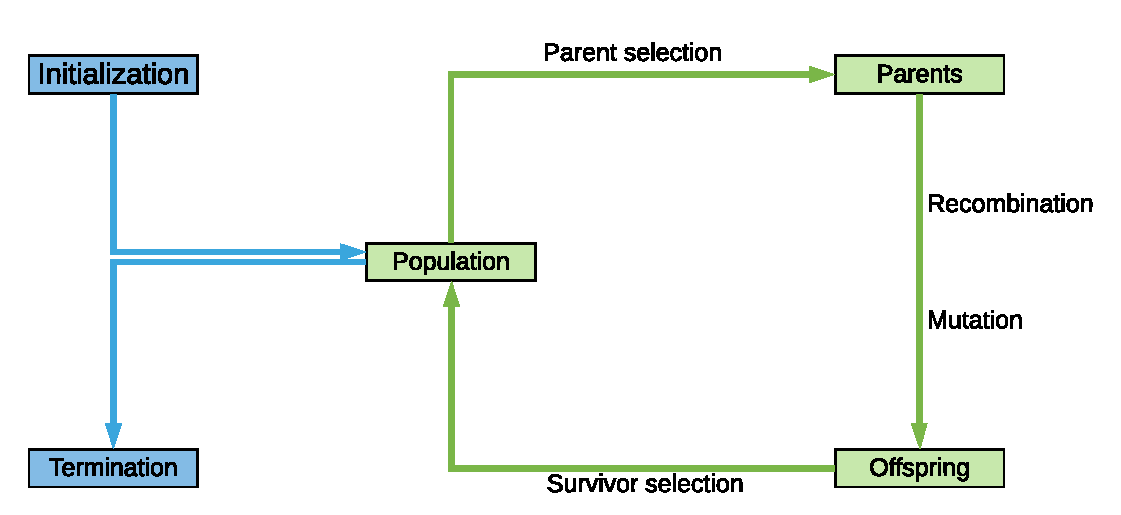
\includegraphics[width=0.9\linewidth]{ea_flowchart}
		\caption[Genereller Ablauf von \gls{ea}s]{Genereller Ablauf von \gls{ea}s (Nachbildung der Graphik aus \cite[Seite 27]{eib-smi-ea})}
		\label{fig:ea-flowchart}
	\end{figure}

	Zuerst wird eine Population - also eine Menge von Individuen (fortwährend als \textit{Lösungskandidaten} bezeichnet) - i\-ni\-ti\-a\-li\-siert. In der Regel geschieht dies mit Zufallszahlen, sofern keine weiteren Eigenschaften bekannt sind, welche erfüllt werden müssen.\\
	Sodann bilden die einzelnen Lösungskandidaten untereinander Paare (dieser Schritt kann - abhängig vom Algorithmus - entfallen).
	
	%Das einzige Unterscheidungsmerkmal der Klassen von \gls{ea}s besteht in der Repräsentation der einzelnen Mitglieder in der Population. 
	%\footnote{mögliche Darstellungsformen sind - wie in \cite{eib-smi-ea} beschrieben - Strings (\textbf{Genetische Algorithmen}), Vektoren von (reellen) Zahlen (\textbf{Evolutionsstrategien}) und Baumstrukturen (\textbf{Genetische Programmierung}) sowie endliche Automaten (\textbf{Evolutionäre Programmierung})}
	
	Vorrangig werden \gls{ea}

	\glsreset{de}

	\section{\gls{de}}
	\label{sec:de}

		Wie in Abschnitt \ref{sec:evol} bereits angedeutet, reiht sich \gls{de} in die \gls{ea} ein. Der von Rainer Storn und Kenneth Price \cite{storn-price-de} 